\documentclass[aspectratio=169]{beamer}

% --- THEME AND STYLING ---
\usetheme{Madrid}
\useoutertheme{default}
\useinnertheme{rectangles}
\setbeamertemplate{navigation symbols}{}

% --- CUSTOM COLOR PALETTE ---
\definecolor{SkyBlue}{RGB}{135, 206, 235}
\definecolor{DarkNavy}{RGB}{0, 0, 139}
\definecolor{LightBlueBg}{RGB}{240, 248, 255}
\definecolor{AccentBlue}{RGB}{70, 130, 180}
\definecolor{DarkGreyText}{RGB}{50, 50, 50}
\definecolor{HighlightGreen}{RGB}{34, 139, 34}
\definecolor{AlertRed}{RGB}{220, 20, 60}

\setbeamercolor{palette primary}{bg=SkyBlue,fg=DarkNavy}
\setbeamercolor{palette secondary}{bg=DarkNavy,fg=white}
\setbeamercolor{palette tertiary}{bg=AccentBlue,fg=white}
\setbeamercolor{palette quaternary}{bg=SkyBlue,fg=DarkNavy}
\setbeamercolor{structure}{fg=DarkNavy}
\setbeamercolor{section in toc}{fg=DarkNavy}
\setbeamercolor{frametitle}{bg=SkyBlue,fg=DarkNavy}
\setbeamercolor{block title}{bg=DarkNavy,fg=white}
\setbeamercolor{block body}{bg=LightBlueBg,fg=DarkGreyText}
\setbeamercolor{block title alerted}{bg=AlertRed,fg=white}
\setbeamercolor{block body alerted}{bg=LightBlueBg,fg=DarkGreyText}
\setbeamercolor{block title example}{bg=HighlightGreen,fg=white}
\setbeamercolor{block body example}{bg=LightBlueBg,fg=DarkGreyText}
\setbeamertemplate{footline}[frame number]
\setbeamercolor{footline}{fg=DarkNavy}
\setbeamertemplate{blocks}[rounded][shadow=false]

% --- PACKAGES ---
\usepackage[utf8]{inputenc}
\usepackage{amsmath,amssymb}
\usepackage{booktabs}
\usepackage{graphicx}
\usepackage{array}
\usepackage{multirow}
\usepackage{tikz}
\usetikzlibrary{positioning}
\usepackage{siunitx}
\usepackage{xcolor}
\usepackage{colortbl}

% --- TITLE PAGE ---
\title[Sustainable Rendezvous]{Sustainable ``Rendezvous'': A Festival Systems Challenge}
\subtitle{End-Semester Presentation --- Modules 3.1\,--\,3.5 (Computational Results)}
\author[Team Sustainability]{Sustainability Task Force}
\institute{Department of Chemical Engineering\\
\vspace{0.2cm}
\small Course: CLL782 -- Process Optimization\\
\small Instructor: Prof.\ Om Prakash}
\date{\today}

\begin{document}

% ================================================================
%  TITLE
% ================================================================
\begin{frame}[plain]
    \titlepage
\end{frame}

% ================================================================
%  PROBLEM STATEMENT
% ================================================================

\begin{frame}{Problem Statement}
    \begin{alertblock}{The Challenge}
        \textbf{``Rendezvous''} --- IIT Delhi's annual cultural festival --- draws \textbf{40{,}000+} visitors over 3 days onto a 163-acre campus not designed for that load.
        \vspace{0.1cm}

        \textit{How do we plan the festival's sustainability infrastructure --- waste bins, collection vehicles, and water stations --- optimally?}
    \end{alertblock}

    \vspace{0.15cm}

    \begin{columns}[T]
        \begin{column}{0.48\textwidth}
            \begin{block}{Sub-Problems (Modules 3.1--3.5)}
                \begin{enumerate}
                    \item[\textbf{3.1}] Environmental load modelling
                    \item[\textbf{3.2}] \textbf{3-type} dustbin placement (FLP)
                    \item[\textbf{3.3}] Waste logistics with \textbf{vehicle segregation}
                    \item[\textbf{3.4}] Water refill station planning (P-Median)
                    \item[\textbf{3.5}] Integrated multi-objective optimization
                \end{enumerate}
            \end{block}
        \end{column}
        \begin{column}{0.48\textwidth}
            \begin{exampleblock}{What Makes This Different}
                \begin{itemize}
                    \item Real \textbf{geospatial data} --- not textbook distances
                    \item \textbf{OSM walking network} + Dijkstra
                    \item Gravity-model footfall estimation
                    \item 3-type waste \& vehicle segregation
                    \item LP relaxation bounds for every module
                \end{itemize}
            \end{exampleblock}
        \end{column}
    \end{columns}
\end{frame}

% ================================================================
%  OUTLINE
% ================================================================
\begin{frame}{Outline}
    \tableofcontents[hideallsubsections]
\end{frame}

% ================================================================
\section{1. Geospatial Data Pipeline (Our USP)}
% ================================================================

\begin{frame}{From Google Earth to MILP: The Geospatial Pipeline}
    \vspace{-0.3cm}
    \begin{center}
    
\begin{tikzpicture}[
        node distance=0.35cm and 0.15cm,
        box/.style={rectangle, rounded corners, draw=DarkNavy, fill=LightBlueBg,
                     text width=2.8cm, minimum height=0.75cm, align=center,
                     font=\footnotesize\bfseries},
        arrow/.style={->, thick, DarkNavy}
    ]
        \node[box] (kml) {Google Earth\\KML Polygon\\{\scriptsize 18 vertices}};
        \node[box, right=of kml] (grid) {UTM Grid\\Generation\\{\scriptsize 50m $\times$ 50m}};
        \node[box, right=of grid] (osm) {OSM Network\\Download\\{\scriptsize 413 nodes, 1078 edges}};
        \node[box, right=of osm] (dijkstra) {Dijkstra's\\Shortest Path\\{\scriptsize 287 $\times$ 287 matrix}};

        \draw[arrow] (kml) -- (grid);
        \draw[arrow] (grid) -- (osm);
        \draw[arrow] (osm) -- (dijkstra);
    \end{tikzpicture}
    \end{center}

    \vspace{-0.1cm}
    \begin{columns}[T]
        \begin{column}{0.50\textwidth}
            \begin{block}{Why Not Just Use Euclidean Distance?}
                \small
                \begin{itemize}\setlength\itemsep{0pt}
                    \item Euclidean \textbf{underestimates by $\sim$30\%} (buildings, fences)
                    \item Real paths follow \textbf{sidewalks \& footpaths}
                    \item Dijkstra on OSM = actual pedestrian reachability
                    \item Every $D_{ij}$ in Mods 3.2--3.5 is a \textbf{real walking distance}
                \end{itemize}
            \end{block}
        \end{column}
        \begin{column}{0.45\textwidth}
            \centering
            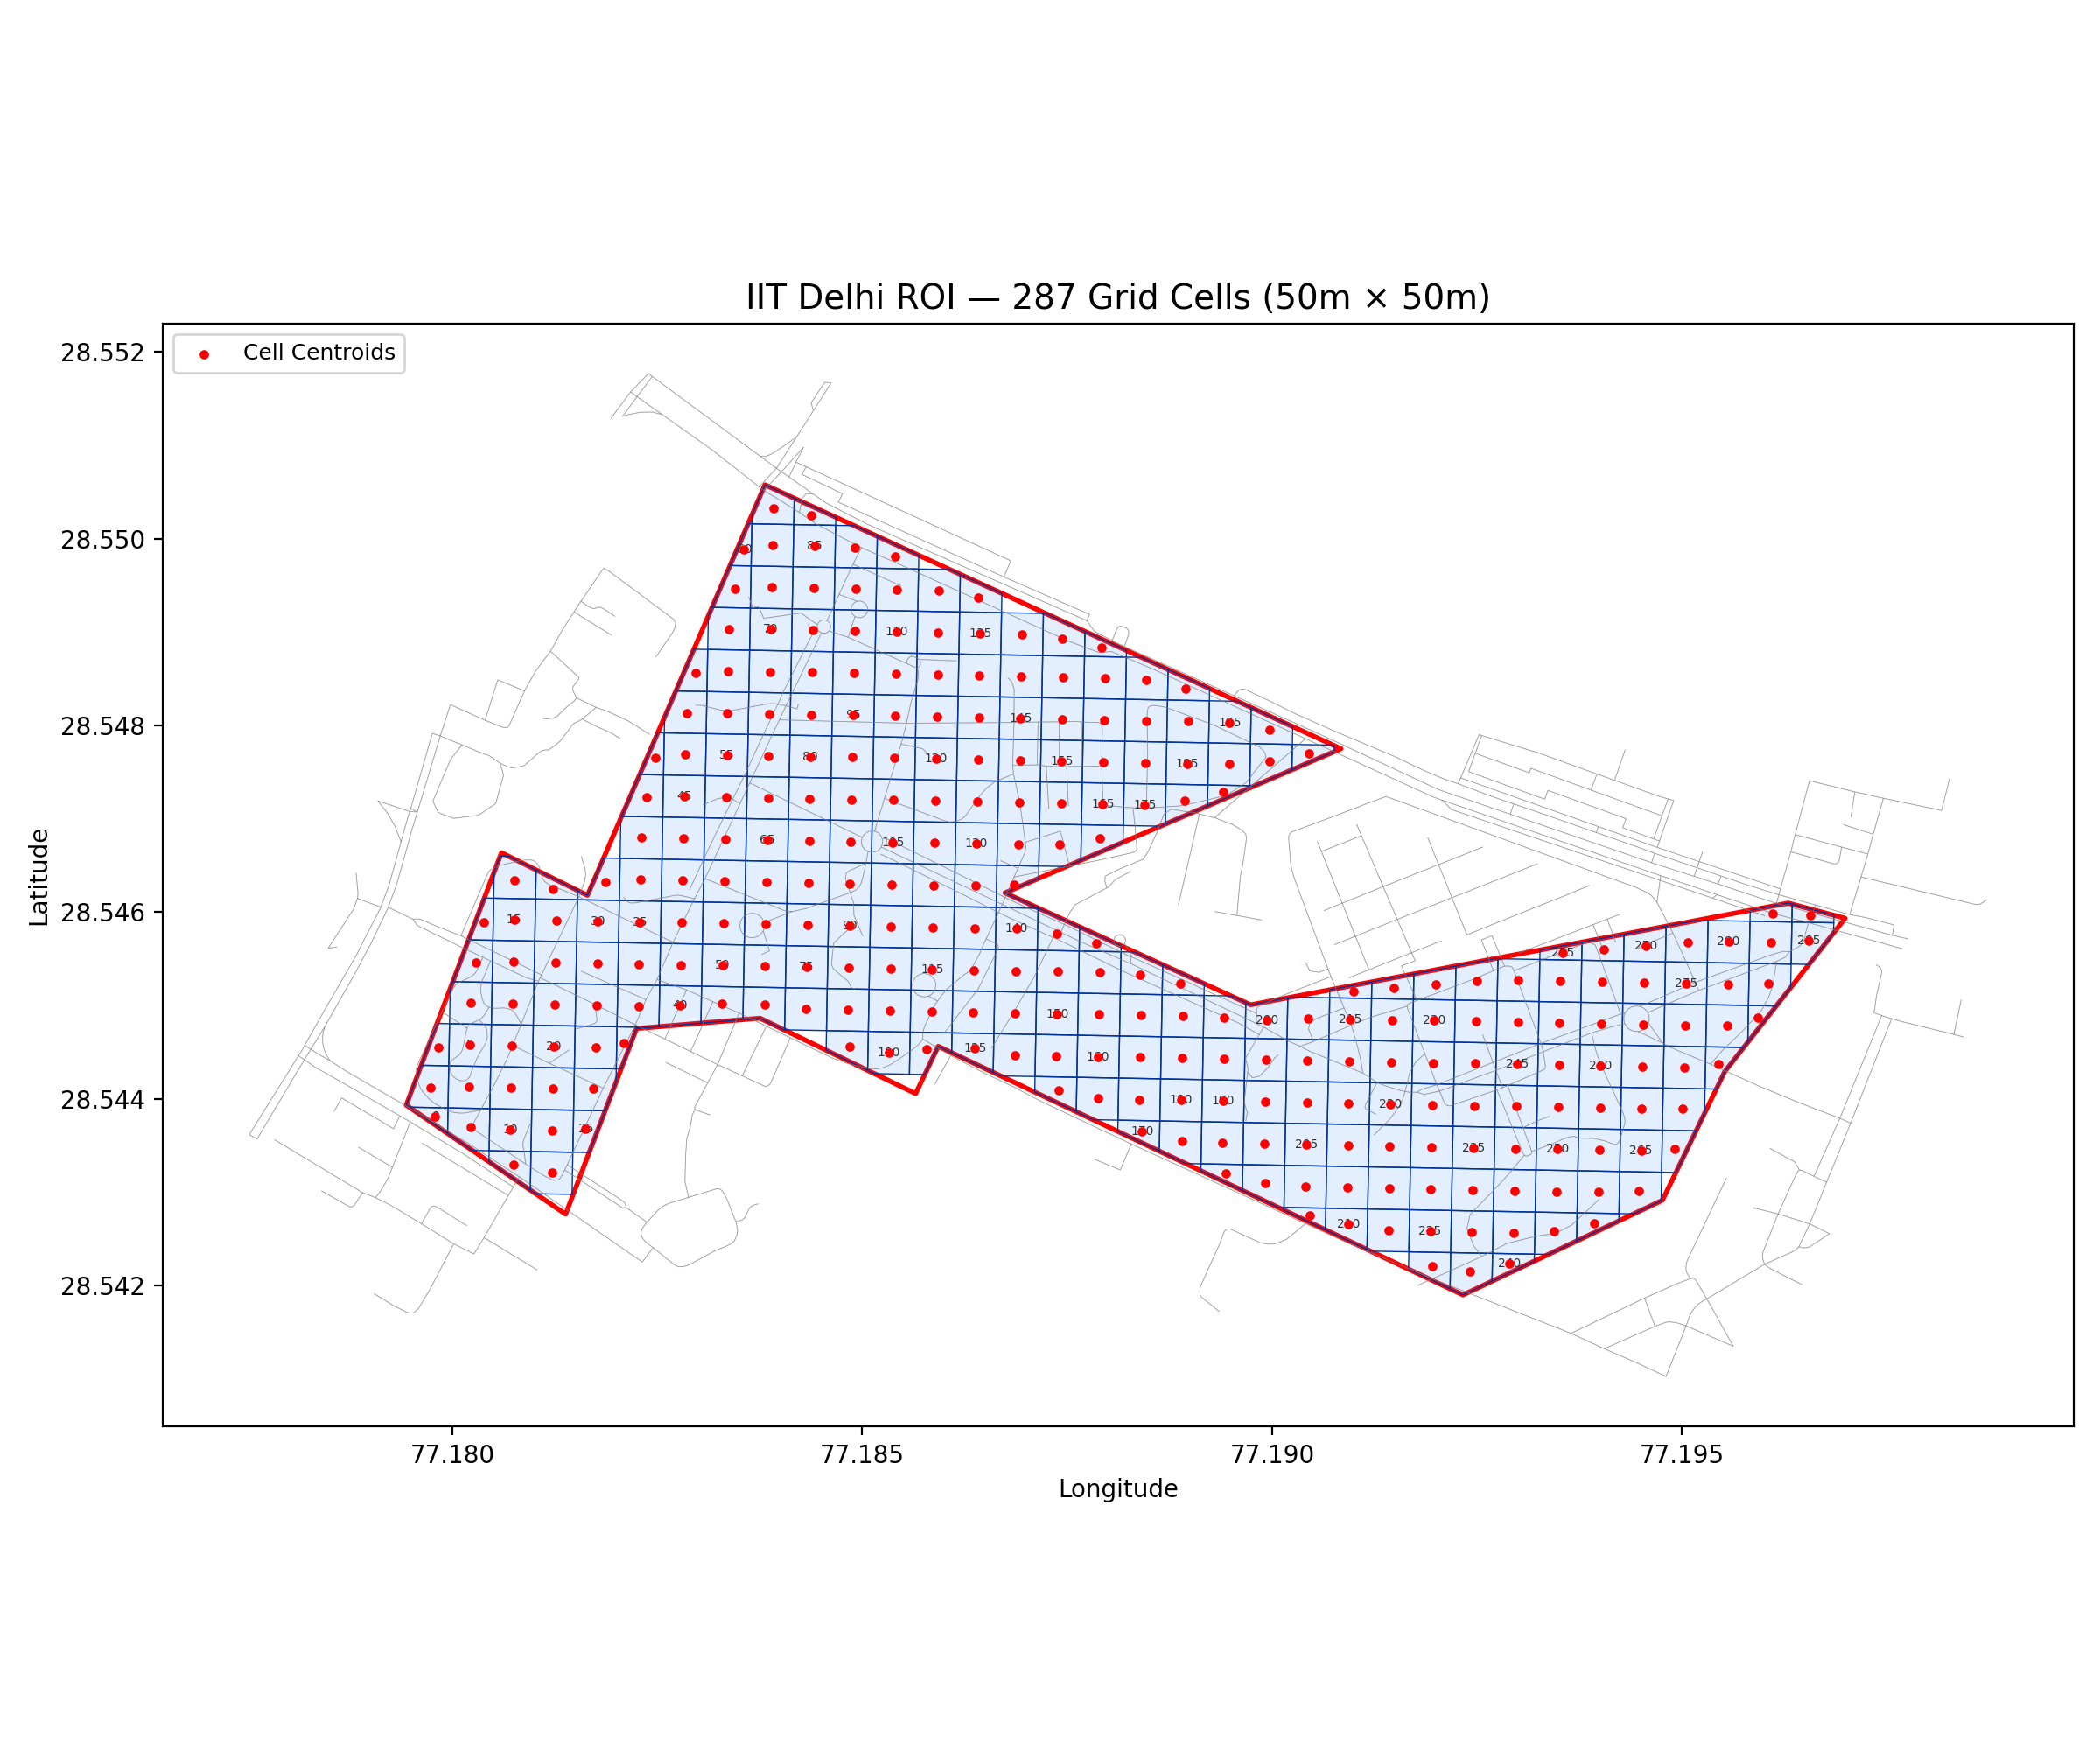
\includegraphics[width=\textwidth]{../grid_data/iitd_roi_grid_map.png}\\
            \tiny{287 grid cells, OSM network (blue), centroids (red) on IIT Delhi campus}
        \end{column}
    \end{columns}
\end{frame}

\begin{frame}{Geospatial Pipeline: Step-by-Step Details}
    \small
    \begin{columns}[T]
        \begin{column}{0.48\textwidth}
            \begin{block}{Step 1: ROI Extraction}
                \begin{itemize}\setlength\itemsep{0pt}
                    \item 18-vertex polygon from Google Earth KML
                    \item \textbf{162.8 acres} (OAT, Nalanda, SAC, LHC, Sports Complex)
                    \item Projected to \textbf{UTM} for metric gridding
                \end{itemize}
            \end{block}

            \begin{exampleblock}{Step 2: Grid Generation}
                \begin{itemize}\setlength\itemsep{0pt}
                    \item 50m $\times$ 50m cells in UTM projection
                    \item Cells with $<$25\% ROI overlap discarded
                    \item \textbf{287 valid cells}: each is both a demand zone $i$ and candidate site $j$
                \end{itemize}
            \end{exampleblock}
        \end{column}
        \begin{column}{0.48\textwidth}
            \begin{alertblock}{Step 3: OSM Walking Network}
                \begin{itemize}\setlength\itemsep{0pt}
                    \item Downloaded via \texttt{osmnx} (ROI + 200m buffer)
                    \item \textbf{413 nodes}, \textbf{1{,}078 edges} (footpaths, roads)
                    \item Each cell centroid \textbf{snapped} to nearest node
                \end{itemize}
            \end{alertblock}

            \begin{block}{Step 4: Walking Distance Matrix}
                \begin{itemize}\setlength\itemsep{0pt}
                    \item Single-source Dijkstra from every snapped node
                    \item 287 $\times$ 287 symmetric matrix
                    \item Avg: \textbf{836.9m}, Max: \textbf{3{,}351m}
                    \item Fallback: Euclidean $\times$ 1.3 if disconnected
                \end{itemize}
            \end{block}
        \end{column}
    \end{columns}

    \vspace{0.1cm}
    \centering
    \textbf{Output}: \texttt{walking\_distance\_matrix.csv} --- the $D_{ij}$ feeding \textbf{every} MILP module.
\end{frame}

\begin{frame}{Footfall \& Waste: Spatial Gravity Model}
    \begin{columns}[T]
        \begin{column}{0.50\textwidth}
            \begin{block}{Gravity Model for Footfall Distribution}
                $$ F_i = \frac{\sum_{v=1}^{10} w_v \, e^{-d_{iv}^2/2\sigma^2} \cdot A_i}{\sum_{k=1}^{287}\sum_{v} w_v \, e^{-d_{kv}^2/2\sigma^2} A_k} \times N_{total} $$
                \footnotesize
                \begin{tabular}{r@{ = }l}
                    $F_i$ & footfall in cell $i$ (persons) \\
                    $w_v$ & attractiveness weight of venue $v$ $\in [0.3, 1]$ \\
                    $d_{iv}$ & haversine distance from cell $i$ to venue $v$ (m) \\
                    $\sigma$ & Gaussian decay length-scale = 350 m \\
                    $A_i$ & area of cell $i$ (m$^2$) \\
                    $N_{total}$ & total peak footfall = 40{,}000 persons \\
                \end{tabular}
            \end{block}
        \end{column}
        \begin{column}{0.45\textwidth}
            \begin{alertblock}{3-Type Waste per Cell (CPCB Norms)}
                Waste per person = 0.15 kg/visit. Split:
                \begin{itemize}
                    \item \textcolor{HighlightGreen}{Compostable}: 40\% = 2{,}400 kg/day
                    \item \textcolor{AccentBlue}{Recyclable}: 40\% = 2{,}400 kg/day
                    \item \textcolor{gray}{General}: 20\% = 1{,}200 kg/day
                \end{itemize}
            \end{alertblock}
            \begin{table}
                \centering\footnotesize
                \begin{tabular}{l r}
                    \toprule
                    \textbf{Metric} & \textbf{Value} \\ \midrule
                    Peak Footfall & 40{,}000 \\
                    Min Cell Footfall & 2.6 persons \\
                    Max Cell Footfall & 288.5 persons \\
                    Total Waste & 6{,}000 kg/day \\
                    \bottomrule
                \end{tabular}
            \end{table}
        \end{column}
    \end{columns}
\end{frame}

% ================================================================
\section{2. Module 3.1: Environmental Load}
% ================================================================

\begin{frame}{3.1 Environmental Load Function}
    \begin{alertblock}{Model: Total Environmental Load $E$ (kg CO$_2$-eq)}
        $$ E(N,S,A) = \underbrace{(\alpha_1 N + \alpha_2 S + \alpha_3 A)}_{\text{Base Load}} + \underbrace{(\beta_N N^{1.3} + \beta_S S^{1.2} + \beta_A A^{0.8})}_{\text{Non-linear Scaling}} + \underbrace{\gamma \frac{N^2}{S}}_{\text{Congestion}} $$
    \end{alertblock}

    \begin{columns}[T]
        \begin{column}{0.48\textwidth}
            \footnotesize
            \textbf{Variables:}
            $N$ = attendees, $S$ = food stalls, $A$ = activity-hours.

            \vspace{0.1cm}
            \textbf{Coefficients} (from literature):\;
            \begin{tabular}{r@{$\;=\;$}l r@{$\;=\;$}l}
                $\alpha_1$ & 2.5  & $\beta_N$ & 0.002 \\
                $\alpha_2$ & 18.0 & $\beta_S$ & 0.5   \\
                $\alpha_3$ & 12.0 & $\beta_A$ & 5.0   \\
                          &      & $\gamma$  & 0.0005 \\
            \end{tabular}

            \vspace{0.1cm}
            \textbf{Goal:} Find $S^*$ minimising $E$ at $N{=}40{,}000$, $A{=}50$.
            \begin{exampleblock}{Results}
                $S^* = 201$ stalls; $E^* = 110{,}524$ kg CO$_2$-eq.\\
                Per-capita: 2.76 kg CO$_2$e/person.
            \end{exampleblock}
        \end{column}
        \begin{column}{0.48\textwidth}
            \centering
            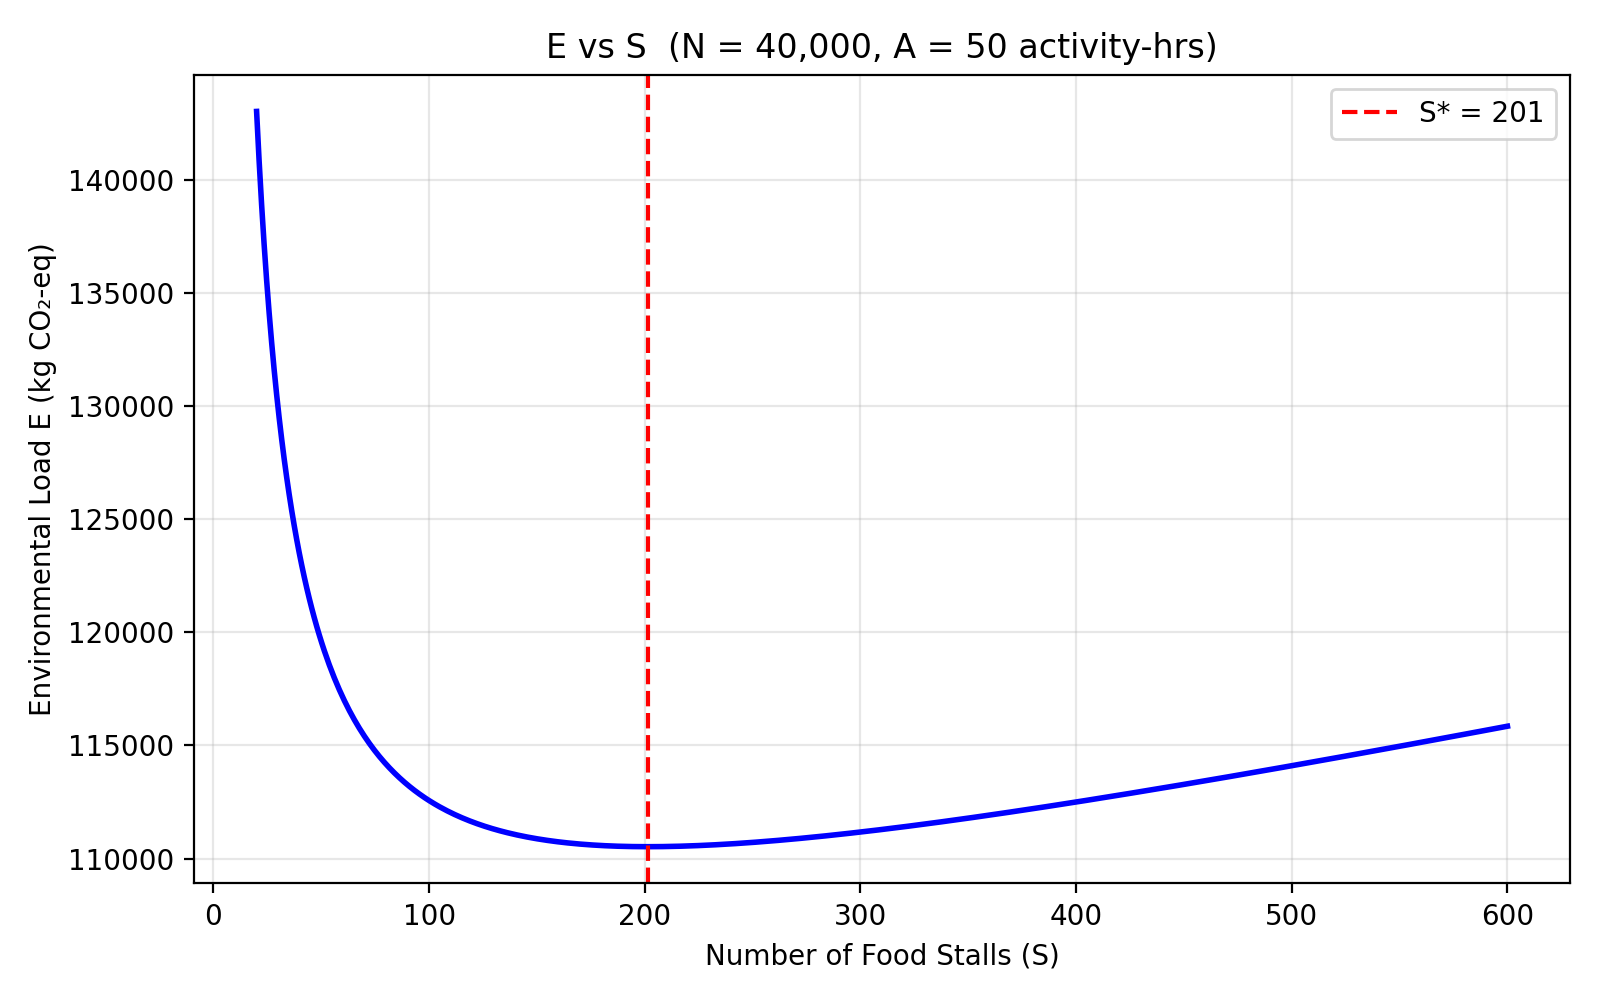
\includegraphics[width=\textwidth]{../Module_3_1/E_vs_S.png}\\
            \tiny{$E$ vs $S$ at fixed $N{=}40{,}000$, $A{=}50$. Minimum at $S^*{\approx}201$.}
        \end{column}
    \end{columns}
\end{frame}

\begin{frame}{3.1 Component Breakdown \& 3D Surface}
    \begin{columns}[T]
        \begin{column}{0.48\textwidth}
            \centering
            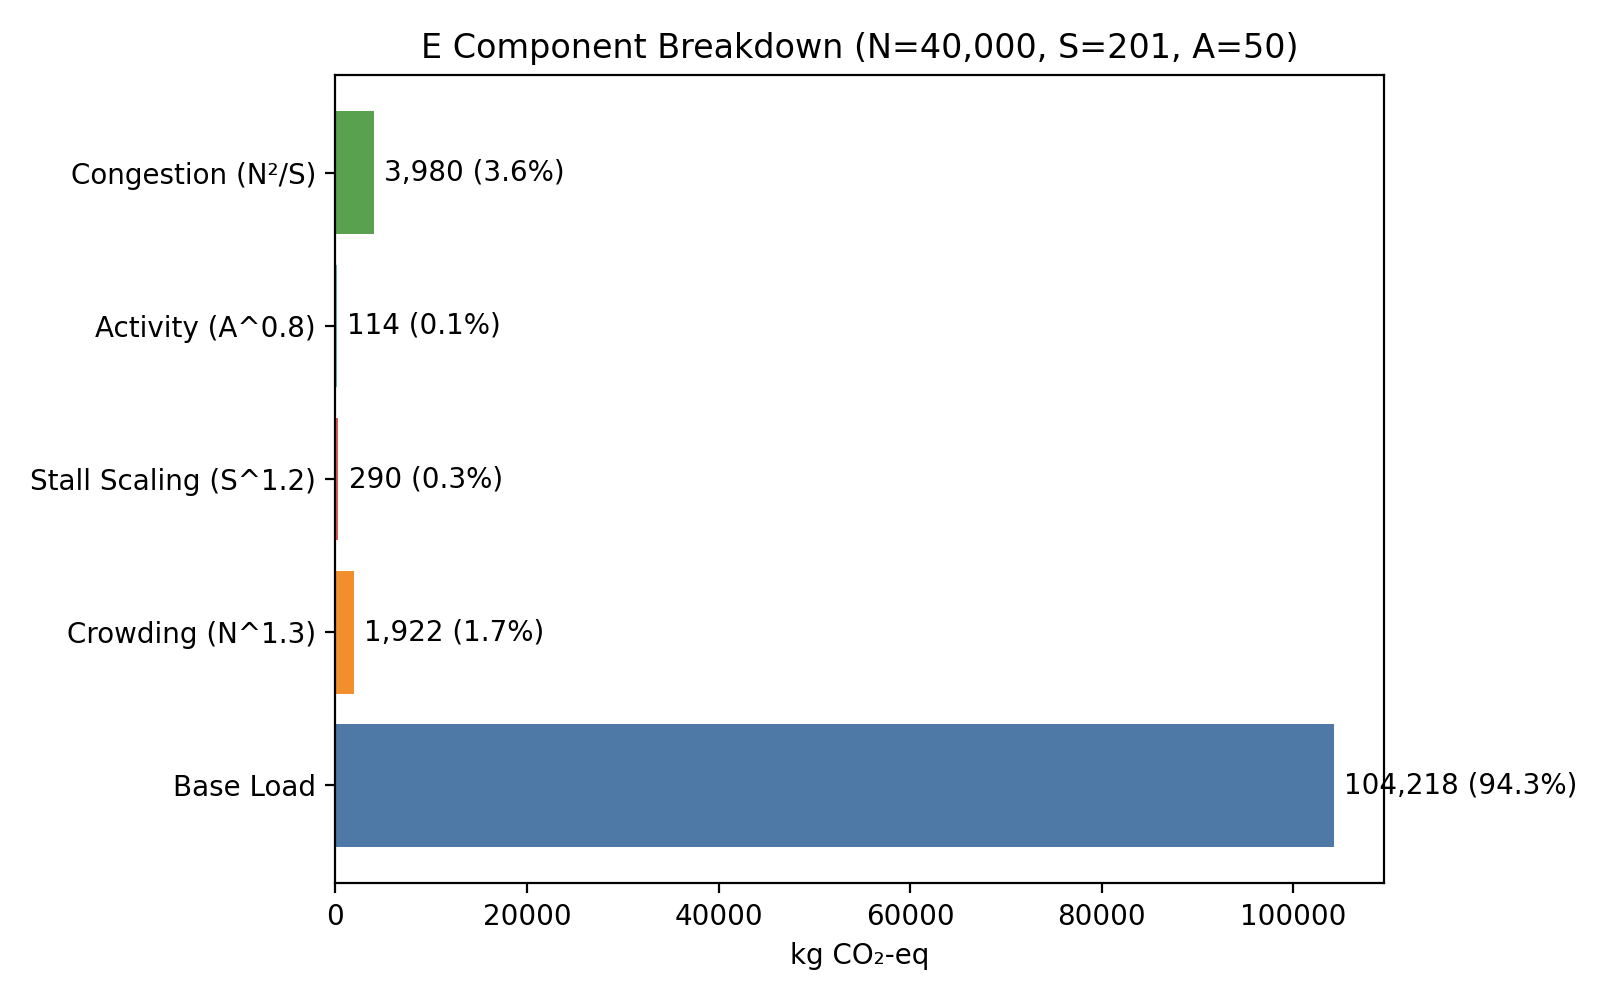
\includegraphics[width=\textwidth]{../Module_3_1/E_breakdown.png}\\
            \tiny{Component decomposition at design point}
        \end{column}
        \begin{column}{0.48\textwidth}
            \centering
            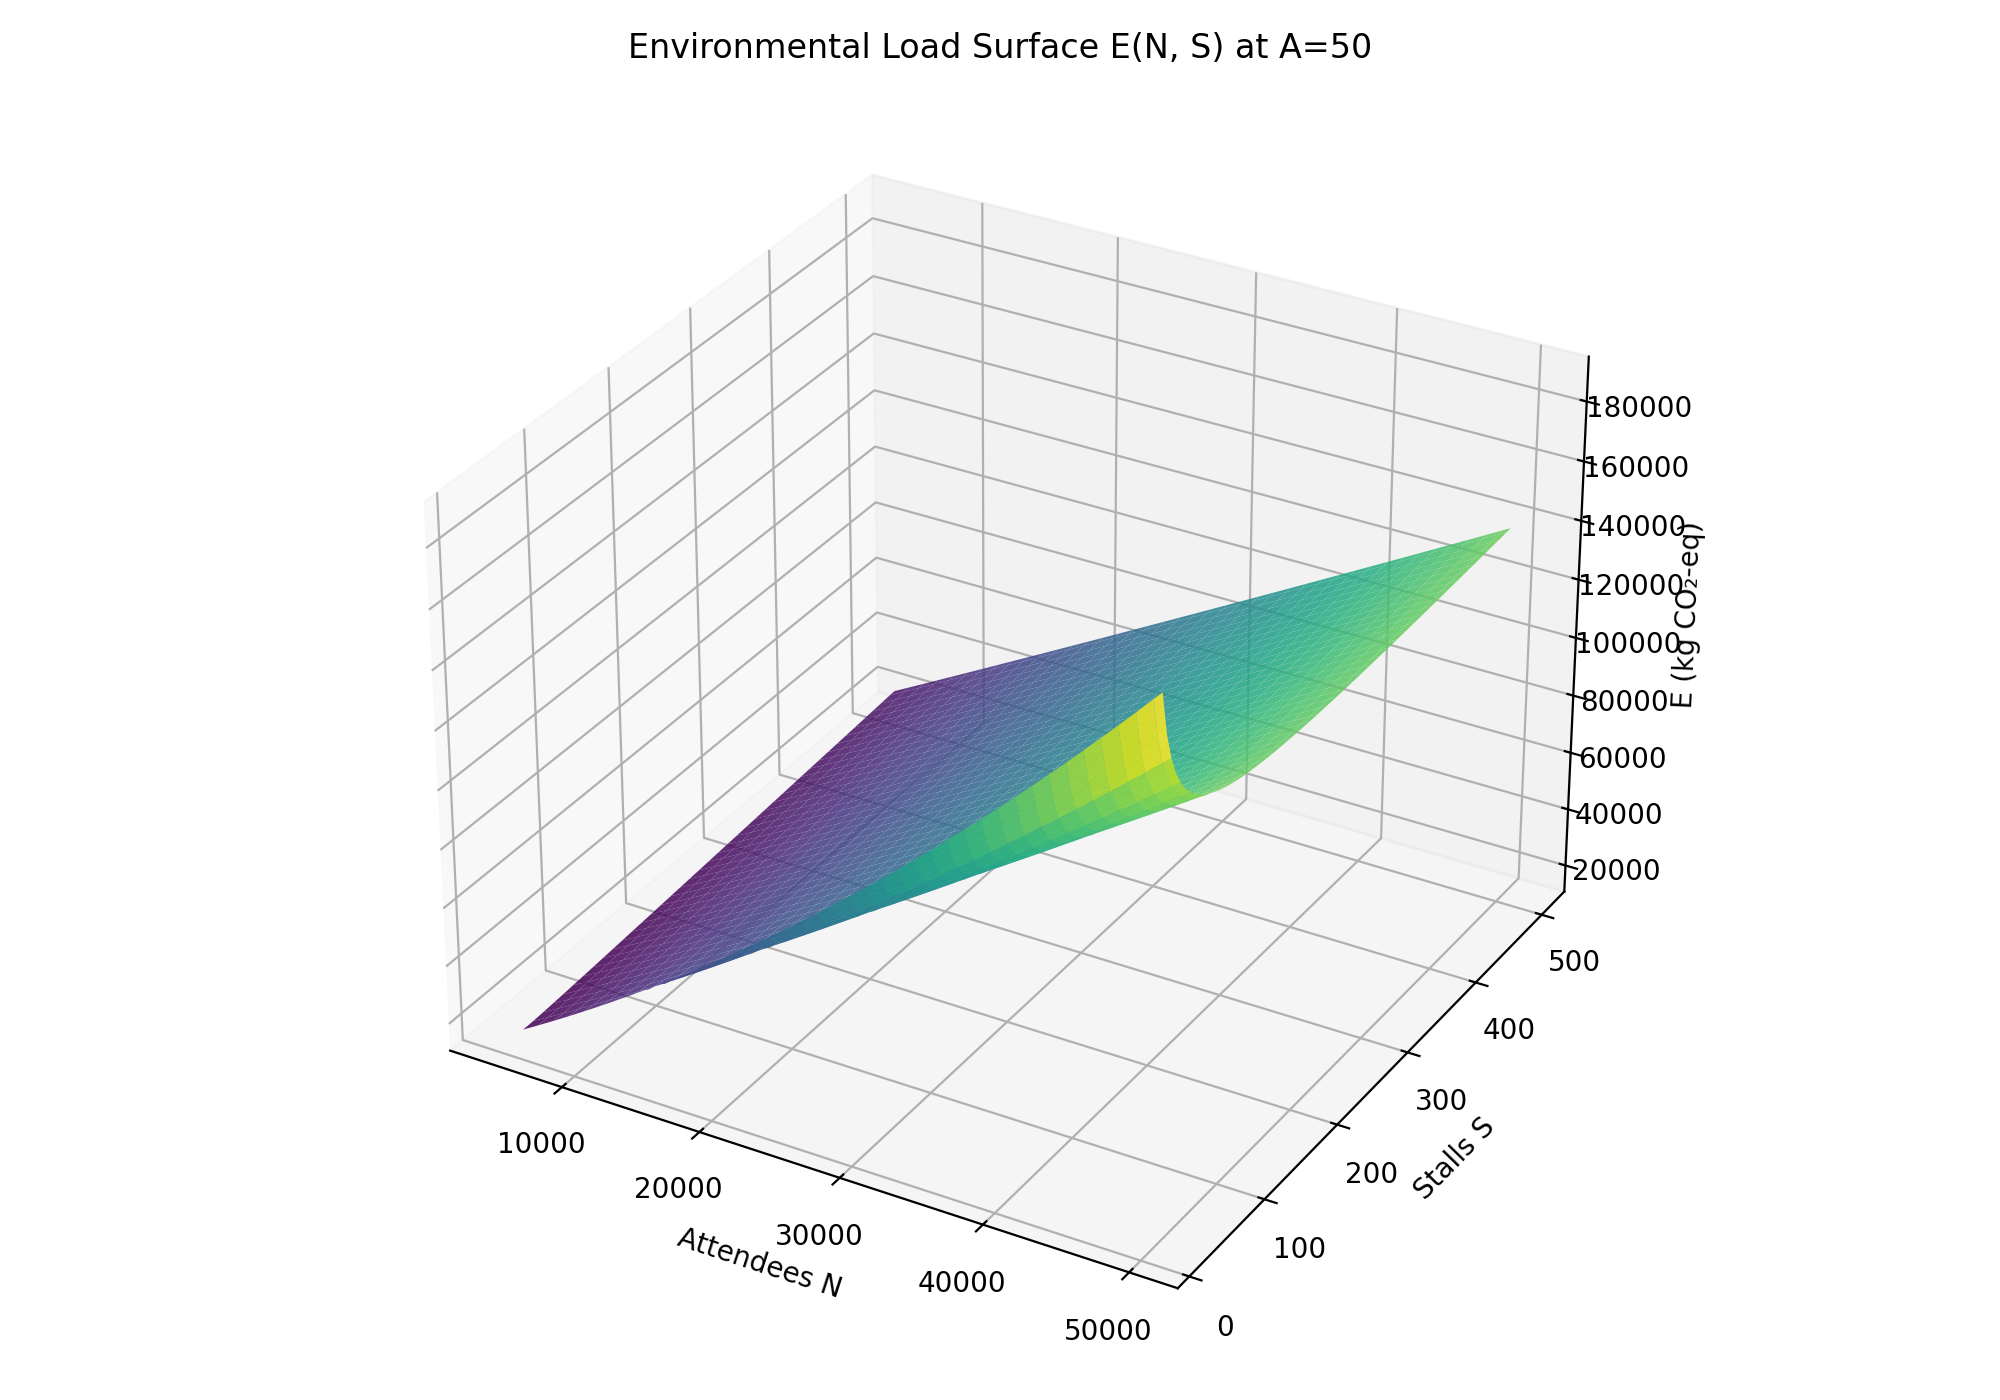
\includegraphics[width=\textwidth]{../Module_3_1/E_surface_NS.png}\\
            \tiny{3D surface: E(N, S) at A=50}
        \end{column}
    \end{columns}
    \vspace{0.2cm}
    \textbf{Insight}: Congestion penalty dominates at low $S$. Base load is the largest single component at the optimum.
\end{frame}

% ================================================================
\section{3. Module 3.2: Dustbin Placement (3-Type Segregation)}
% ================================================================

\begin{frame}{3.2 Formulation: 3-Type Waste-Segregated FLP}
    \begin{block}{Key Change from Midsem}
        \textbf{3 bin types} $t \in \{\text{compostable}, \text{recyclable}, \text{general}\}$ with type-specific capacity, cost, and service radius.
    \end{block}
    \begin{exampleblock}{Decision Variables}
        \begin{itemize}
            \item $y_{j,t} \in \mathbb{Z}_{\ge 0}$: Number of bins of type $t$ at site $j$
            \item $a_{i,j,t} \in [0,1]$: Fraction of zone $i$'s type-$t$ waste assigned to bin $j$
        \end{itemize}
    \end{exampleblock}

    \begin{table}
        \centering\footnotesize
        \begin{tabular}{l c c c c}
            \toprule
            \textbf{Bin Type} & \textbf{Color} & \textbf{Capacity (kg)} & \textbf{Cost (Rs.)} & \textbf{Radius (m)} \\ \midrule
            \rowcolor{green!15} Compostable (Wet) & Green & 20 & 10{,}000 & 200 \\
            \rowcolor{blue!10} Recyclable (Dry) & Blue & 15 & 8{,}000 & 200 \\
            \rowcolor{gray!15} General (Inert) & Grey & 10 & 6{,}000 & 250 \\
            \bottomrule
        \end{tabular}
    \end{table}
\end{frame}

\begin{frame}{3.2 MILP Formulation}
    \begin{alertblock}{Objective: Minimise Total Waste-Weighted Walking Distance}
        $$ \min \; Z = \sum_{i=1}^{287} \sum_{j} \sum_{t \in \mathcal{T}} W_{i,t} \cdot a_{i,j,t} \cdot D_{ij} $$
    \end{alertblock}

    \footnotesize
    \textbf{Where:} $W_{i,t}$ = waste of type $t$ in zone $i$ (kg), \; $D_{ij}$ = walking distance from $i$ to $j$ (m, from Dijkstra), \; $\mathcal{T}$ = \{compostable, recyclable, general\}.

    \vspace{0.15cm}
    \textbf{Subject to:}
    \begin{enumerate}
        \item \textbf{Full coverage}: $\sum_{j} a_{i,j,t} = 1 \;\; \forall\, i, t$ \hfill (every zone's waste assigned)
        \item \textbf{Bin capacity}: $\sum_{i} W_{i,t} \cdot a_{i,j,t} \le K_t \cdot y_{j,t} \;\; \forall\, j, t$ \hfill ($K_t$ = capacity per bin of type $t$, kg)
        \item \textbf{Service radius}: $a_{i,j,t} = 0$ if $D_{ij} > R_t$ \hfill ($R_t$ = max walk to bin type $t$, m)
        \item \textbf{Budget}: $\sum_{j} \sum_{t} C_t \cdot y_{j,t} \le 35{,}00{,}000$ \hfill ($C_t$ = unit cost of bin type $t$, Rs.)
    \end{enumerate}

    \vspace{0.1cm}
    \normalsize
    Solved as MILP using \textbf{PuLP/CBC}. LP relaxation also solved for lower bound.
\end{frame}

\begin{frame}{3.2 Computational Results}
    \begin{columns}[T]
        \begin{column}{0.48\textwidth}
            \begin{block}{MILP Solution}
                \begin{itemize}
                    \item \textcolor{HighlightGreen}{Compostable}: 135 bins at 108 sites
                    \item \textcolor{AccentBlue}{Recyclable}: 172 bins at 120 sites
                    \item \textcolor{gray}{General}: 129 bins at 99 sites
                    \item \textbf{Total: 436 bins}
                    \item Cost: Rs.\,35,00,000 (100\% of budget)
                    \item Objective: 93{,}209 (waste-m)
                \end{itemize}
            \end{block}
            \begin{alertblock}{LP Relaxation}
                Objective = 0 (bins at exact demand sites). \\
                LP lower bound: 400 bins, Rs.\,32,01,440.
            \end{alertblock}
        \end{column}
        \begin{column}{0.48\textwidth}
            \centering
            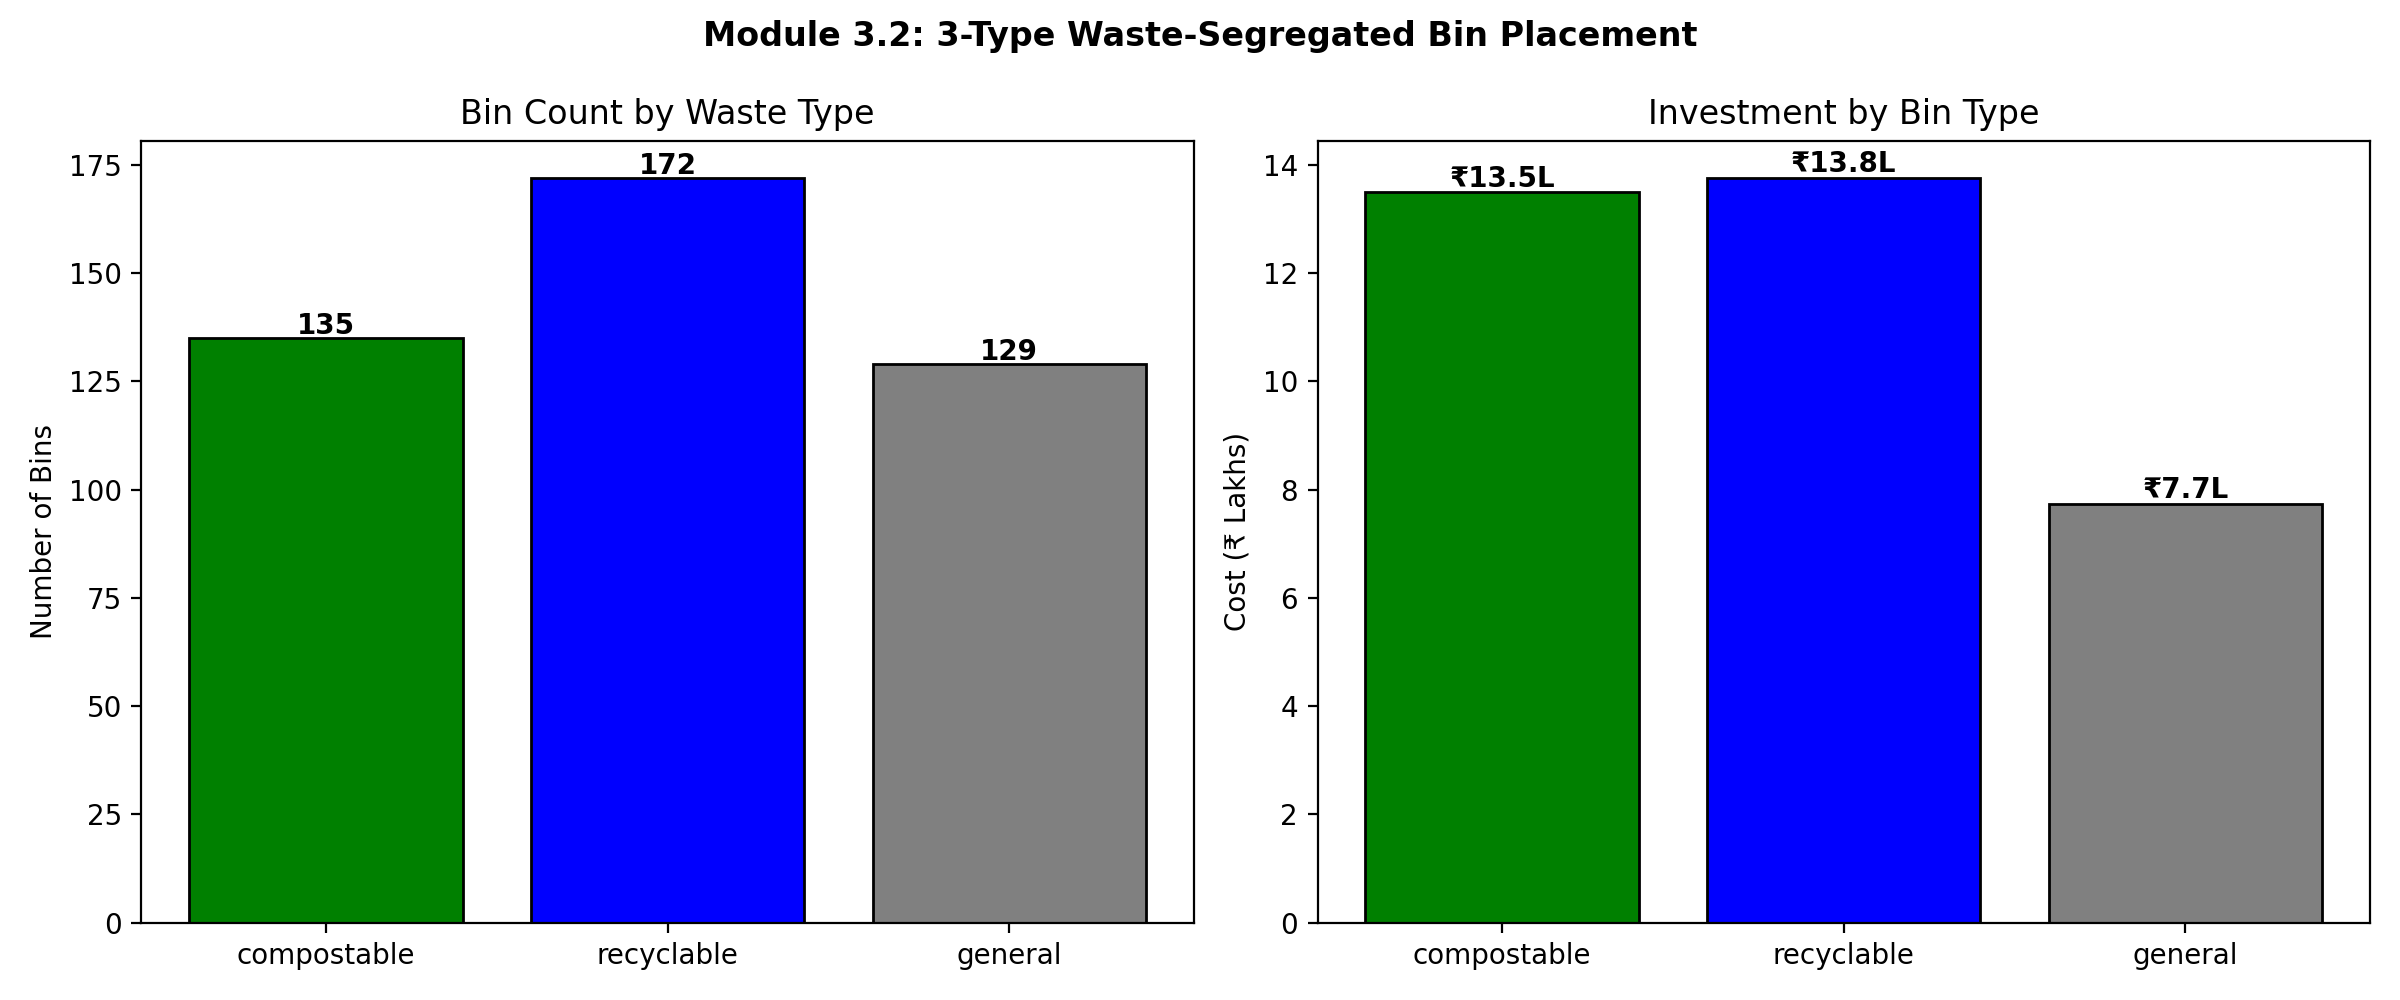
\includegraphics[width=\textwidth]{../Module_3_2/bin_placement_summary.png}\\
            \tiny{Bin counts and cost by waste type}
        \end{column}
    \end{columns}
\end{frame}

% ================================================================
\section{4. Module 3.3: Waste Logistics (Vehicle Type Segregation)}
% ================================================================

\begin{frame}{3.3 Formulation: Vehicle Type Segregation}
    \begin{alertblock}{Objective: Minimise Total Daily Logistics Cost}
        $$ \min \; \sum_{t \in \mathcal{T}} \sum_{i} \sum_{j \in \mathcal{F}_t} \underbrace{\left(c^{var}_t \cdot L_j + c^{hdl} + c^{proc}_j\right)}_{\text{unit cost per kg}} \!\cdot\, x_{i,j,t} \;+\; \sum_{t} c^{fix}_t \cdot N_t $$
    \end{alertblock}

    \footnotesize
    \textbf{Variables:} $x_{i,j,t} \ge 0$ = kg of waste type $t$ shipped from zone $i$ to facility $j$; \;\; $N_t \in \mathbb{Z}_{\ge 0}$ = vehicles of type $t$ deployed. \\
    \textbf{Where:} $c^{var}_t$ = Rs./km for vehicle type $t$; \; $L_j$ = distance to facility $j$ (km); \; $c^{hdl}$ = handling cost (Rs.\,1/kg); \; $c^{proc}_j$ = processing cost at $j$ (Rs./kg); \; $c^{fix}_t$ = daily fixed cost per vehicle; \; $\mathcal{F}_t$ = facilities accepting type $t$.

    \vspace{0.15cm}
    \normalsize
    \begin{columns}[T]
        \begin{column}{0.48\textwidth}
            \begin{table}
                \centering\footnotesize
                \begin{tabular}{l l l}
                    \toprule
                    \textbf{Waste $t$} & \textbf{Facility $j$} & \textbf{$L_j$} \\ \midrule
                    \rowcolor{green!15} Compostable & Biogas (cap 500 kg) & 1 km \\
                    \rowcolor{blue!10} Recyclable & Okhla Recycler & 11 km \\
                    \rowcolor{gray!15} General & Okhla Landfill & 12 km \\
                    \bottomrule
                \end{tabular}
            \end{table}
        \end{column}
        \begin{column}{0.48\textwidth}
            \begin{table}
                \centering\footnotesize
                \begin{tabular}{l c c c}
                    \toprule
                    \textbf{Vehicle} & \textbf{Cap} & $c^{fix}_t$ & $c^{var}_t$ \\ \midrule
                    \rowcolor{green!15} Green Tipper & 750 kg & 600 & 15 \\
                    \rowcolor{blue!10} Blue Tipper & 750 kg & 600 & 15 \\
                    \rowcolor{gray!15} Grey Tipper & 500 kg & 500 & 18 \\
                    \bottomrule
                \end{tabular}
            \end{table}
        \end{column}
    \end{columns}
\end{frame}

\begin{frame}{3.3 Results: Base Scenario}
    \begin{columns}[T]
        \begin{column}{0.48\textwidth}
            \begin{block}{Optimal Flow Allocation}
                \small
                \begin{itemize}\setlength\itemsep{0pt}
                    \item \textcolor{HighlightGreen}{Compostable}: 500 kg $\to$ Biogas, 1{,}900 kg $\to$ Landfill
                    \item \textcolor{AccentBlue}{Recyclable}: 2{,}400 kg $\to$ Recycler
                    \item \textcolor{gray}{General}: 1{,}200 kg $\to$ Landfill
                \end{itemize}
            \end{block}
            \begin{exampleblock}{Cost Breakdown}
                \small
                \begin{itemize}\setlength\itemsep{0pt}
                    \item Transport + Handling: Rs.\,10,10,700
                    \item Processing: $-$Rs.\,12,750 (recycling revenue!)
                    \item Fleet Fixed: Rs.\,3,400
                    \item \textbf{Total: Rs.\,10,01,350}
                \end{itemize}
            \end{exampleblock}
            \small Fleet: 2 Green + 2 Blue + 2 Grey = \textbf{6 vehicles}.
        \end{column}
        \begin{column}{0.48\textwidth}
            \centering
            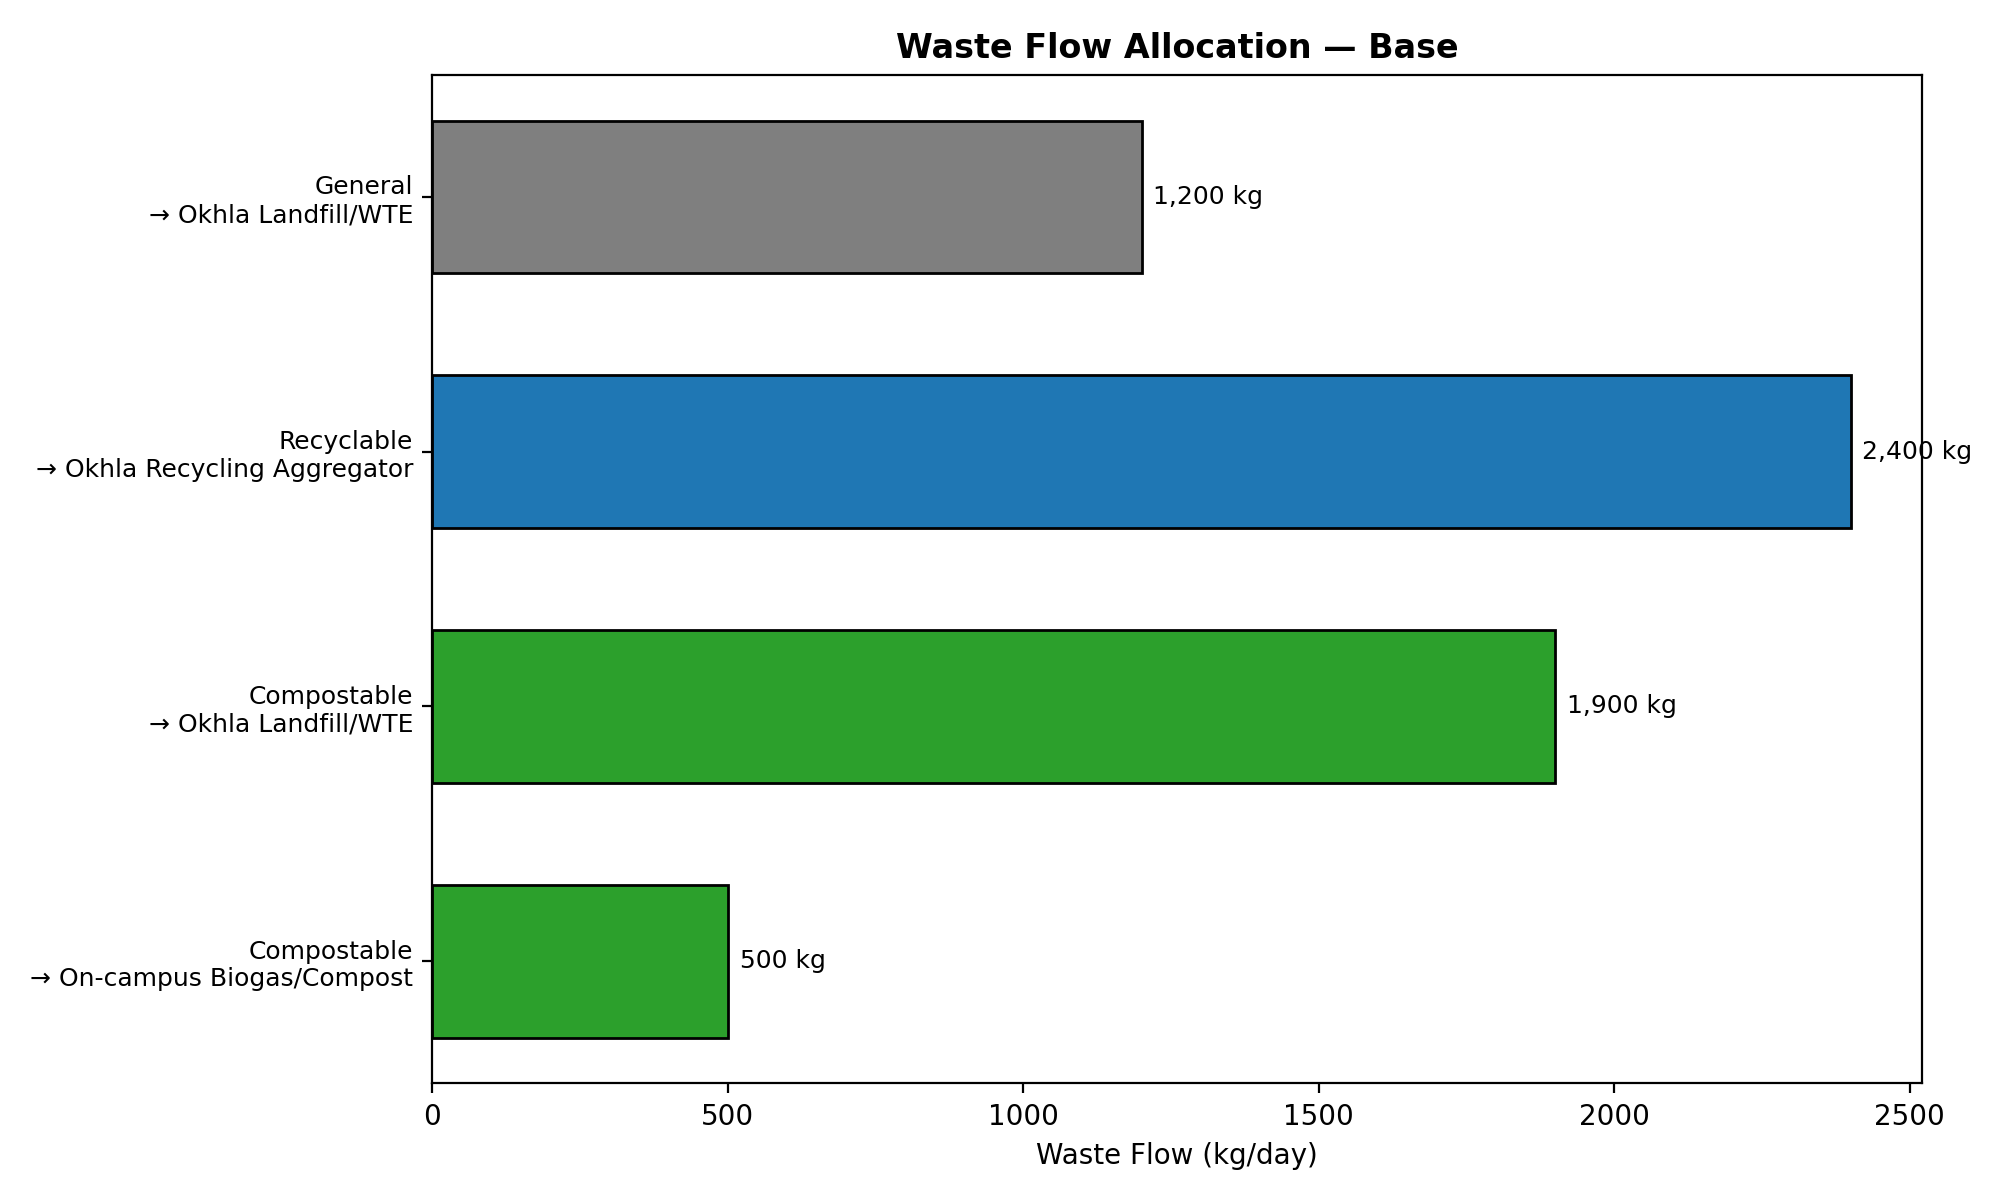
\includegraphics[width=\textwidth]{../Module_3_3/waste_flow_base.png}\\
            \tiny{Waste flow allocation --- base scenario}
        \end{column}
    \end{columns}
\end{frame}

\begin{frame}{3.3 Sensitivity Analysis: +20\% Waste}
    \begin{columns}[T]
        \begin{column}{0.48\textwidth}
            \begin{alertblock}{Key Findings}
                \small
                \begin{itemize}\setlength\itemsep{0pt}
                    \item Biogas at 500 kg cap even in base case.
                    \item \textbf{1{,}900 kg compostable $\to$ landfill} (base); 2{,}380 at $+20\%$.
                    \item Cost: $+21.6\%$ (Rs.\,2,16,240).
                    \item Same fleet size (absorbed by trips).
                    \item \textbf{Bottleneck}: composting capacity.
                \end{itemize}
            \end{alertblock}
        \end{column}
        \begin{column}{0.48\textwidth}
            \centering
            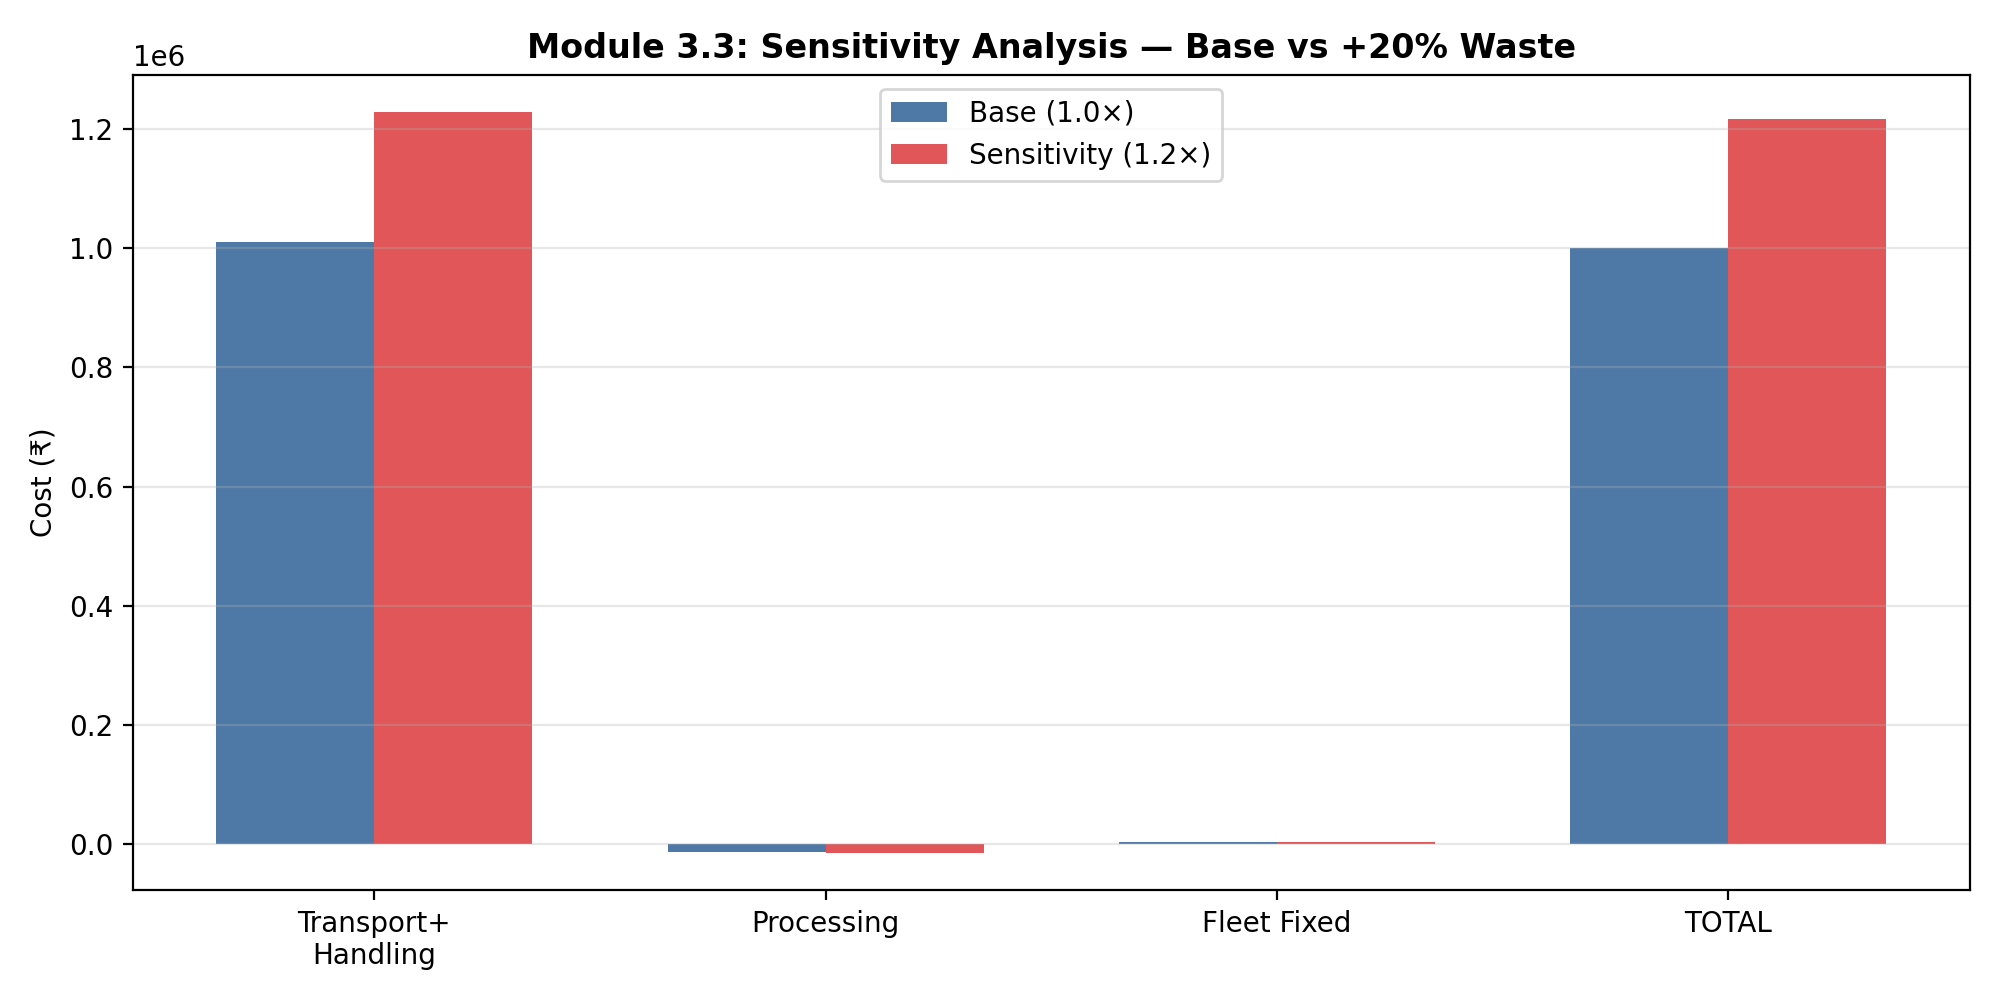
\includegraphics[width=0.88\textwidth]{../Module_3_3/sensitivity_comparison.png}\\[-0.1cm]
            \tiny{Cost comparison: Base vs +20\% waste}\\[0.0cm]
            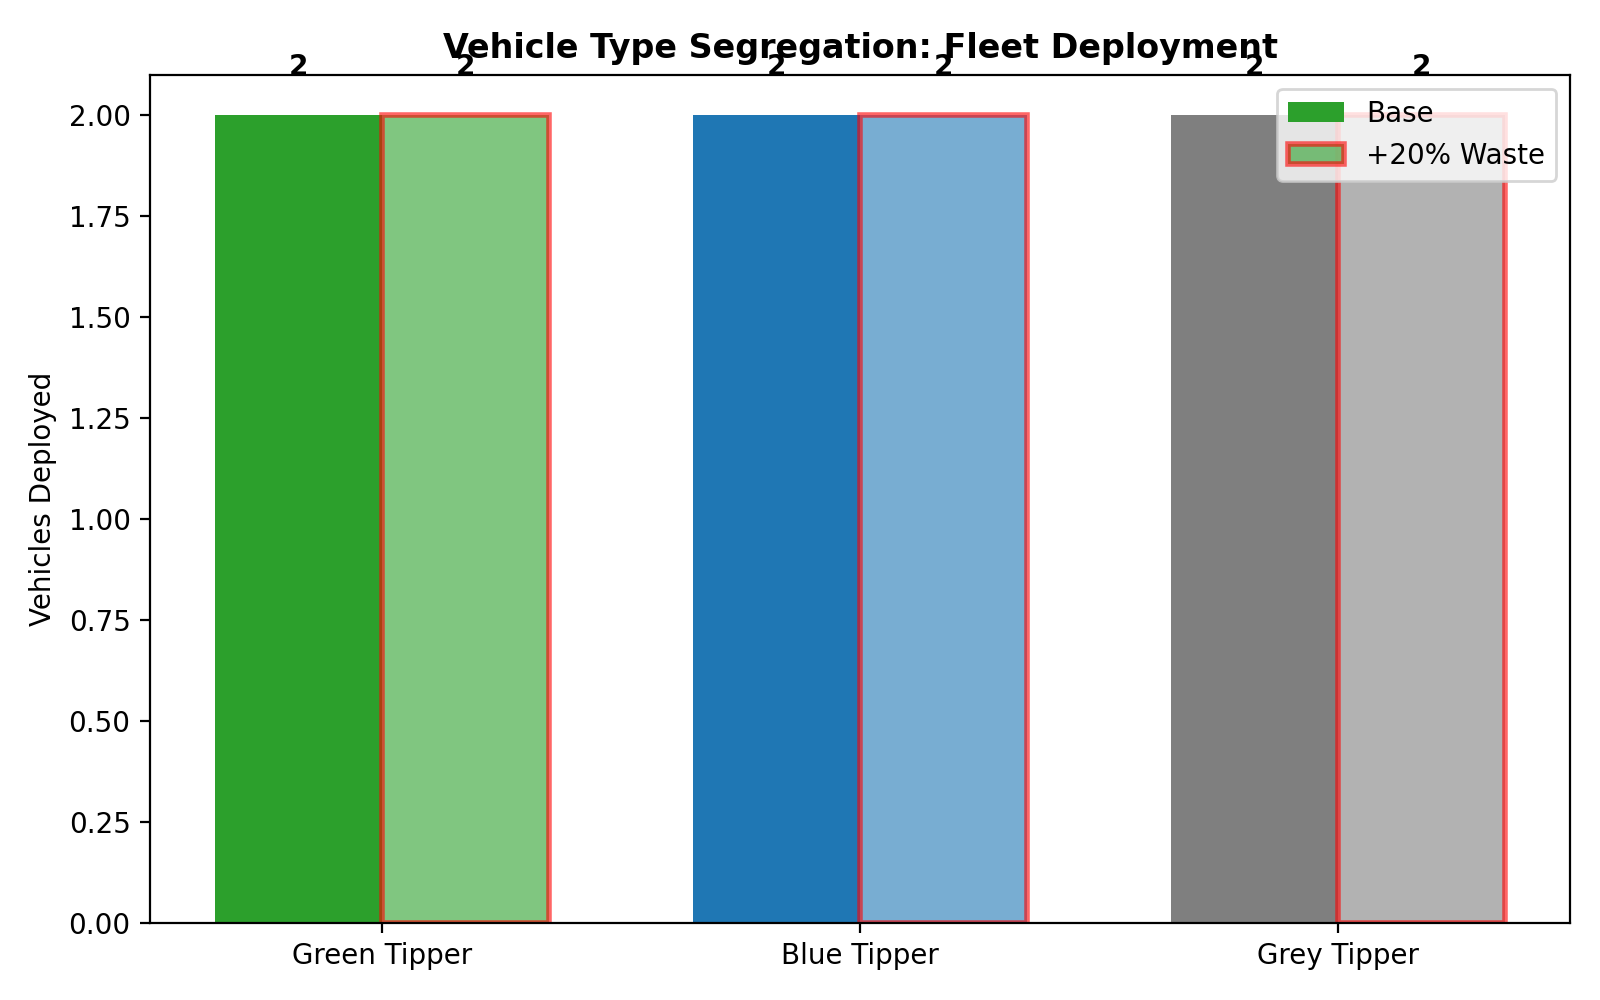
\includegraphics[width=0.88\textwidth]{../Module_3_3/vehicle_deployment.png}\\[-0.1cm]
            \tiny{Vehicle deployment by type}
        \end{column}
    \end{columns}
\end{frame}

% ================================================================
\section{5. Module 3.4: Water Refill Stations}
% ================================================================

\begin{frame}{3.4 Capacitated P-Median: Water Refill Stations}
    \vspace{-0.15cm}
    \begin{alertblock}{Objective}
        \vspace{-0.2cm}
        $$ \min \; \underbrace{\sum_{j} f \cdot y_j}_{\text{Installation}} + \underbrace{\sum_{i,j} F_i \cdot x_{i,j} \cdot D_{ij} \cdot c_w}_{\text{Walking inconvenience}} $$
        \vspace{-0.2cm}
    \end{alertblock}
    \vspace{-0.1cm}
    \begin{columns}[T]
        \begin{column}{0.52\textwidth}
            \scriptsize
            \textbf{Variables:}
            $y_j \in \{0,1\}$: open station at $j$; \;
            $x_{i,j} \in [0,1]$: frac.\ of zone $i$ assigned to $j$.\\[0.05cm]
            \textbf{Parameters:}
            $f{=}$Rs.\,1L/station; \; $F_i{=}$footfall (persons); \; $D_{ij}{=}$walking dist.\ (m); \; $c_w{=}$Rs.\,0.02/m; \; $Q{=}$1{,}000 persons/station.\\[0.05cm]
            \textbf{Constraints:}
            $\sum_j x_{i,j}{=}1\;\forall i$ (demand met); \;
            $\sum_i F_i x_{i,j} {\le}\, Q y_j\;\forall j$ (capacity); \;
            $x_{i,j}{=}0$ if $D_{ij}{>}500$m.
        \end{column}
        \begin{column}{0.44\textwidth}
            \begin{exampleblock}{Results (Greedy + LP Bound)}
                \footnotesize
                \begin{itemize}\setlength\itemsep{0pt}
                    \item \textbf{40 stations}, Rs.\,40{,}00{,}000
                    \item Avg walk: \textbf{75 m}, Max: 2{,}492 m
                    \item Capacity = demand = 10{,}000 LPH
                    \item \textbf{LP gap: 1.31\%}
                \end{itemize}
            \end{exampleblock}
        \end{column}
    \end{columns}
\end{frame}

% ================================================================
\section{6. Module 3.5: Integrated System Model}
% ================================================================

\begin{frame}{3.5 Multi-Objective Optimization}
    \vspace{-0.15cm}
    \begin{alertblock}{Formulation: Budget-Constrained Weighted Sum}
        \vspace{-0.2cm}
        $$ \min_{B_{bin},\, B_{stn}} \;\; w_1 \hat{C}_{sys} + w_2 \hat{E}_{sys} + w_3 \hat{I}_{sys} \qquad \text{s.t. } B_{bin} + B_{stn} \le B_{total} = \text{Rs.\,85L} $$
        \vspace{-0.3cm}
    \end{alertblock}
    \vspace{-0.1cm}
    \scriptsize
    \textbf{Decision Variables:} $B_{bin}$ = bin budget; $B_{stn}$ = station budget. \quad \textbf{Weights:} $w_1 + w_2 + w_3 = 1$, swept over simplex.\\
    \textbf{Objectives} ($\hat{(\cdot)}$ = min-max normalised to $[0,1]$):
    $C_{sys}$ = total economic cost (Rs.); \;
    $E_{sys}$ = CO$_2$e from infrastructure + waste processing (kg); \;
    $I_{sys}$ = walking inconvenience (person$\cdot$m$\cdot$Rs.). \; Solved via SciPy SLSQP (multi-start).

    \normalsize
    \begin{columns}[T]
        \begin{column}{0.48\textwidth}
            \begin{table}
                \centering\footnotesize
                \begin{tabular}{l r r}
                    \toprule
                    & \textbf{Min Cost} & \textbf{Min Inconv.} \\ \midrule
                    Bins & 404 & 535 \\
                    Stations & 40 & 40 \\
                    $C_{sys}$ & Rs.\,83.9L & Rs.\,95.0L \\
                    $E_{sys}$ & 6{,}690 CO$_2$e & 7{,}345 CO$_2$e \\
                    $I_{sys}$ & 160{,}657 & 136{,}026 \\
                    \bottomrule
                \end{tabular}
            \end{table}
        \end{column}
        \begin{column}{0.48\textwidth}
            \begin{exampleblock}{Recommended (Balanced)}
                \small
                Weights: $w_1{=}0.29,\; w_2{=}0.31,\; w_3{=}0.41$
                \begin{itemize}\setlength\itemsep{0pt}
                    \item \textbf{404 bins} + \textbf{40 stations}
                    \item Bins Rs.\,34L + Stations Rs.\,40.8L
                    \item Total: Rs.\,83.9L, CO$_2$e: 6{,}690 kg
                \end{itemize}
            \end{exampleblock}
        \end{column}
    \end{columns}
\end{frame}

\begin{frame}{3.5 Pareto Frontier \& Budget Allocation}
    \begin{columns}[T]
        \begin{column}{0.48\textwidth}
            \centering
            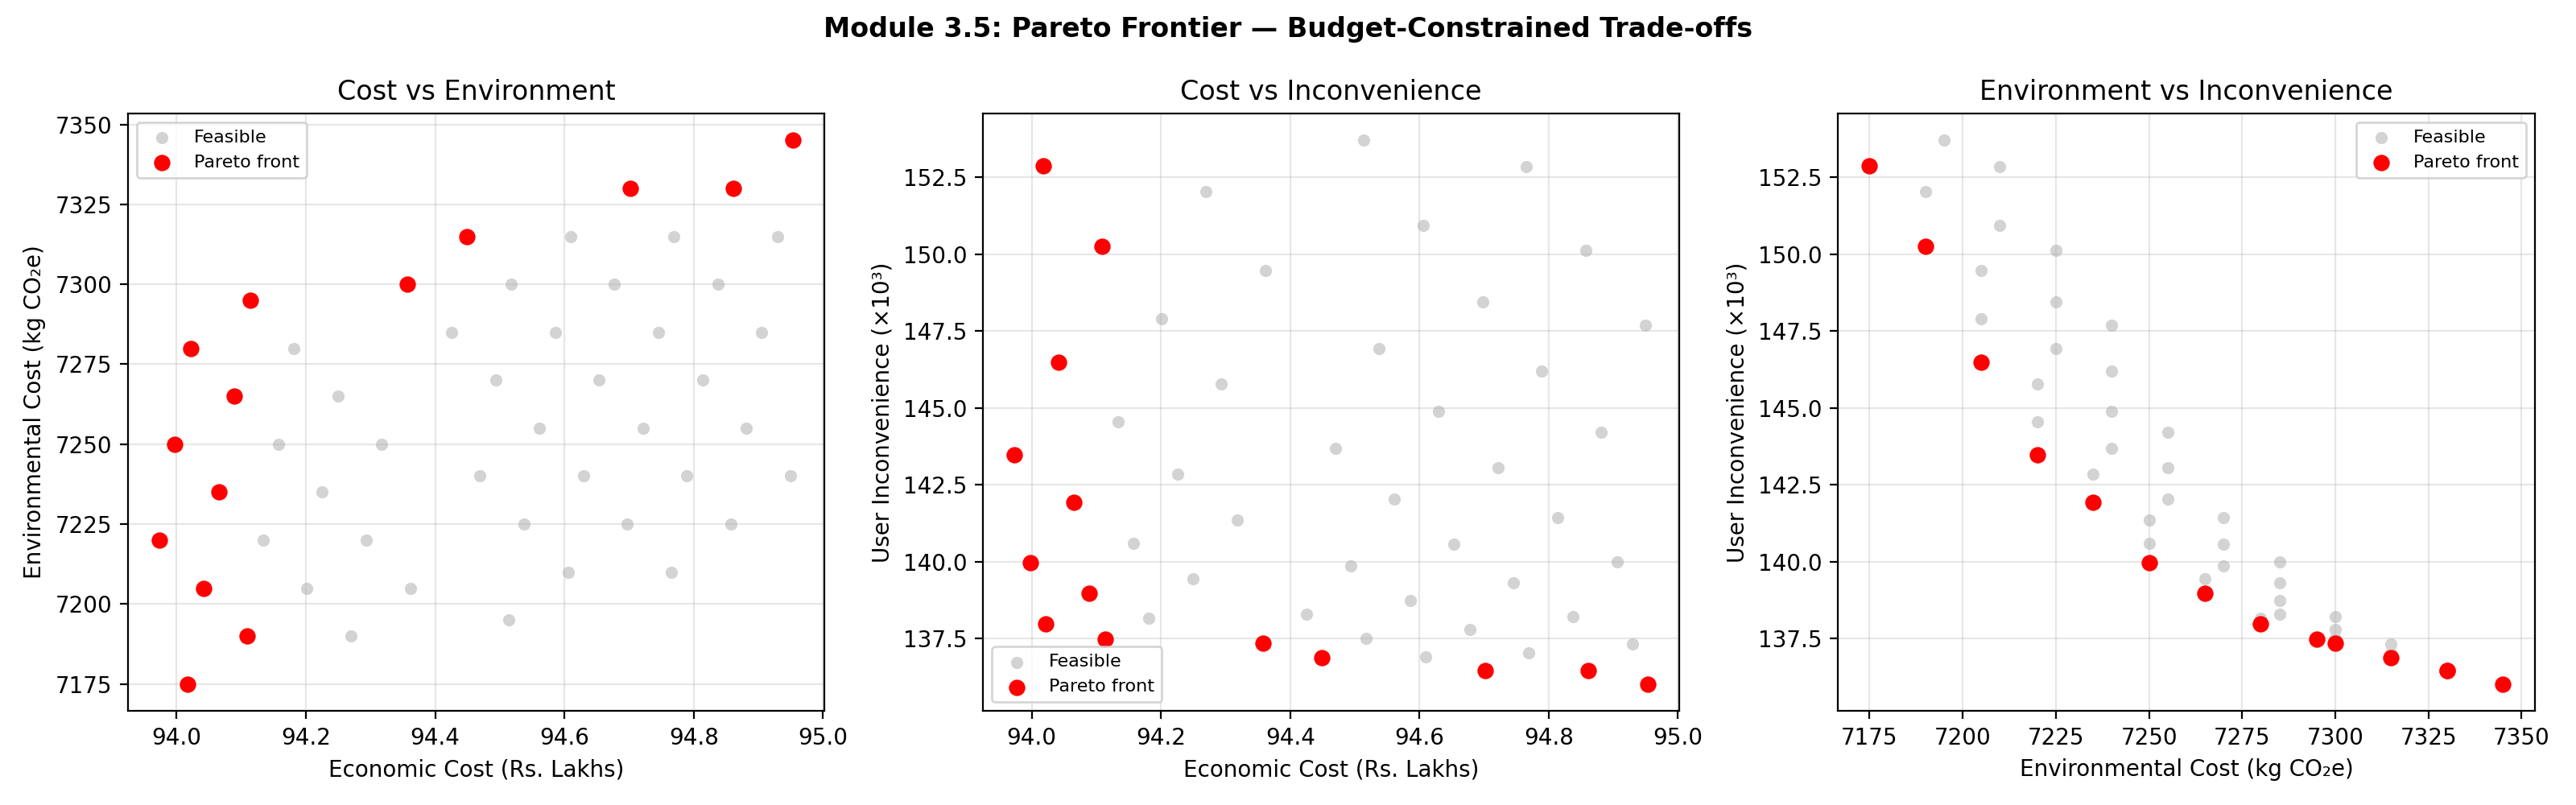
\includegraphics[width=\textwidth]{../Module_3_5/pareto_frontier_3d.png}\\
            \tiny{Pareto frontier: Cost vs Environment vs Inconvenience}
        \end{column}
        \begin{column}{0.48\textwidth}
            \centering
            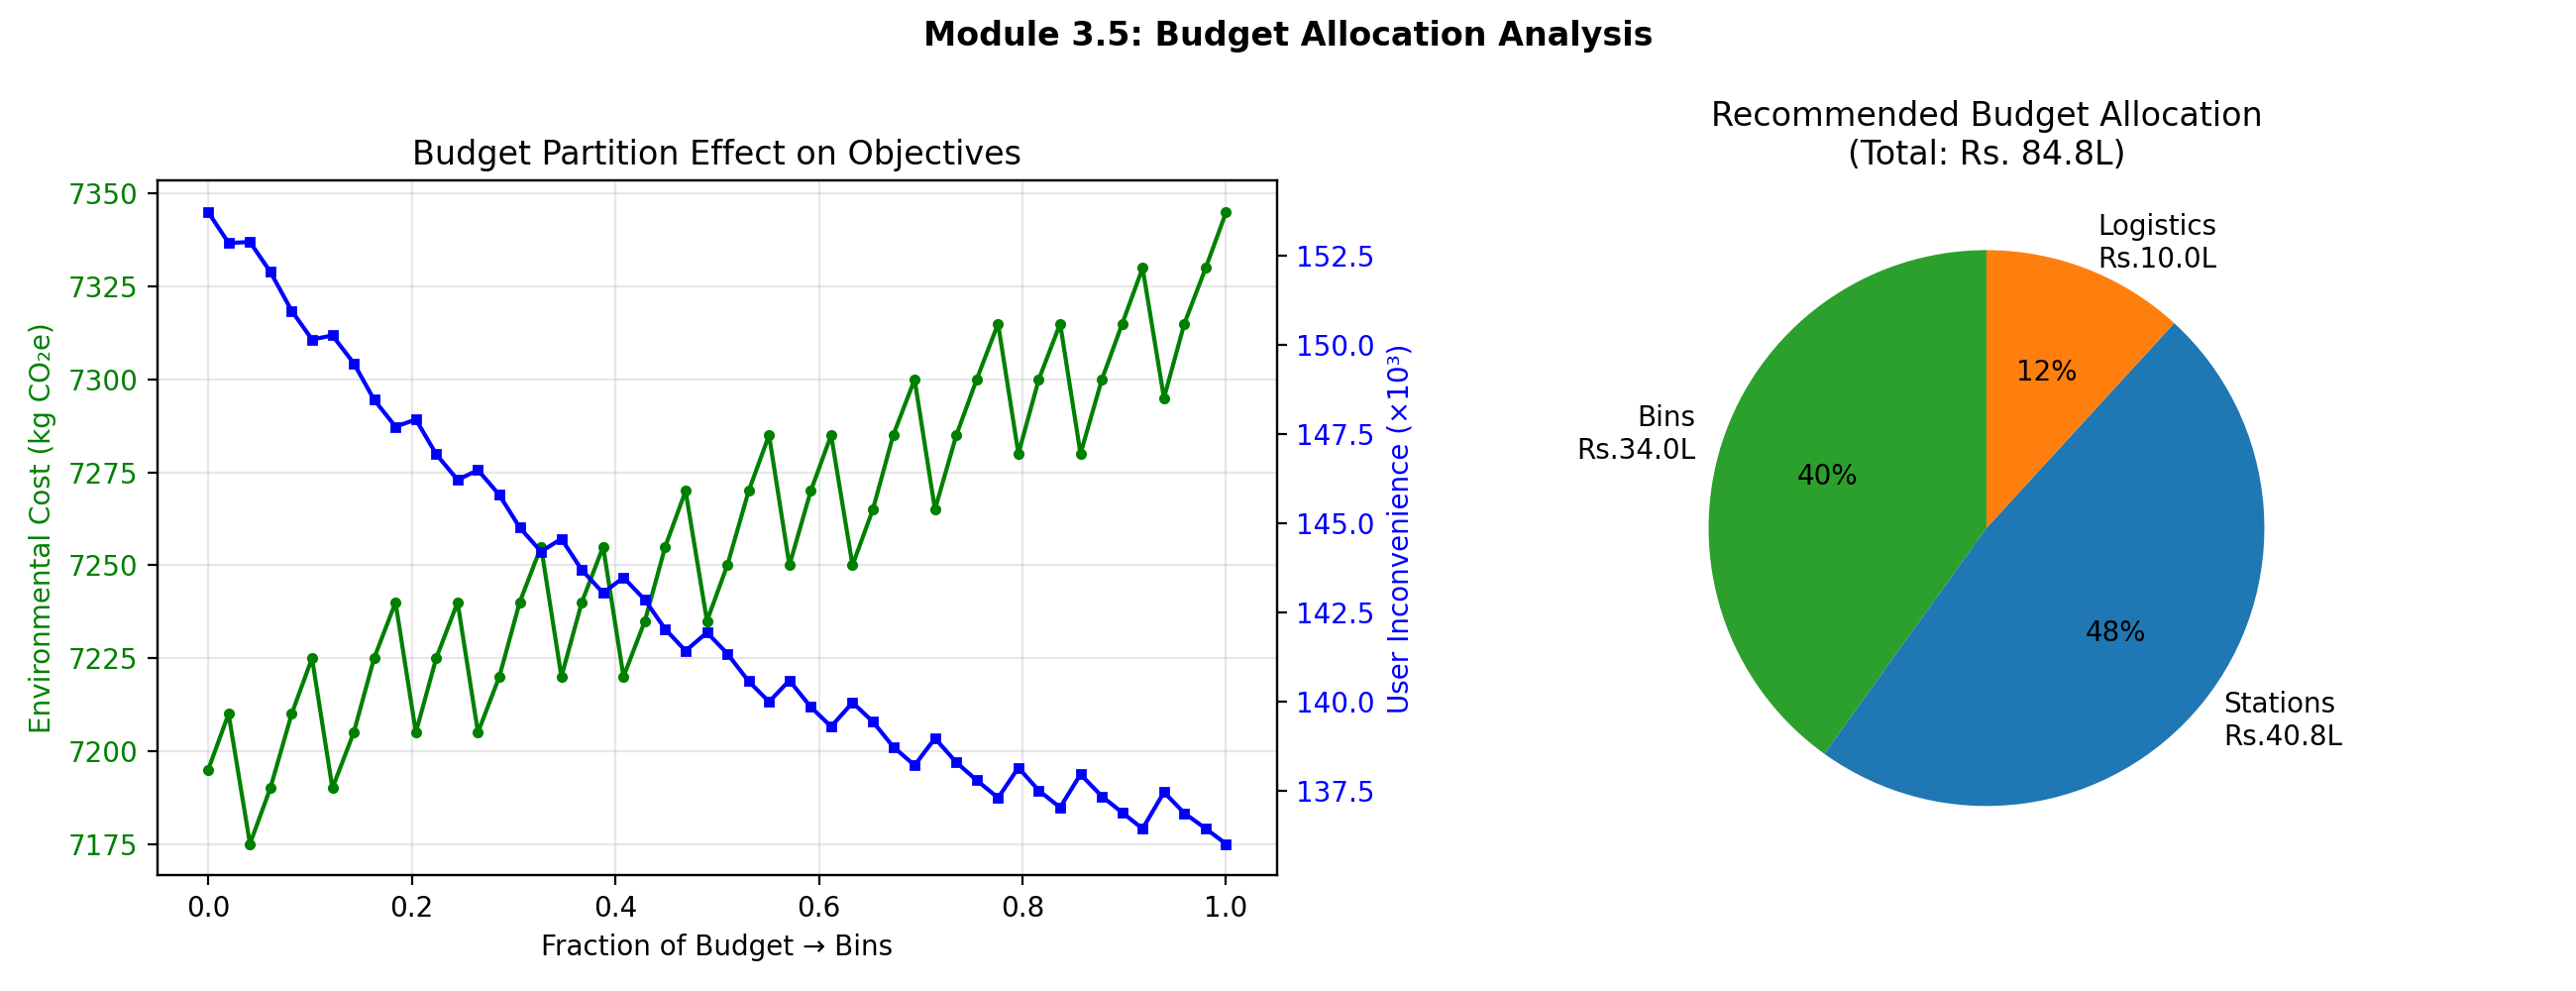
\includegraphics[width=\textwidth]{../Module_3_5/tradeoff_2d.png}\\
            \tiny{Budget partition effects and recommended allocation}
        \end{column}
    \end{columns}
    \vspace{0.1cm}
    \small
    \textbf{Key Insights}:
    \begin{itemize}\setlength\itemsep{1pt}
        \item Stations always at minimum (40) --- capacity constraint is tight.
        \item Extra bin budget yields diminishing returns on inconvenience.
        \item \textbf{Expanding composting capacity} would shift the Pareto frontier favourably.
    \end{itemize}
\end{frame}

% ================================================================
\section{Conclusion}
% ================================================================

\begin{frame}{Integrated Blueprint \& Key Takeaways}
    \begin{block}{System-Level Summary}
        \begin{enumerate}
            \item \textbf{Mod 3.1}: $S^* \approx 201$ stalls; $E = 110{,}524$ kg CO$_2$-eq at design point.
            \item \textbf{Mod 3.2}: \textbf{436 bins} (3 types) across 287 zones; full waste segregation at source.
            \item \textbf{Mod 3.3}: \textbf{6 segregated vehicles} (Green/Blue/Grey); biogas bottleneck at 500 kg/day.
            \item \textbf{Mod 3.4}: \textbf{40 refill stations}; avg walk 75m; LP gap 1.31\%.
            \item \textbf{Mod 3.5}: Budget-constrained Pareto frontier; balanced point at Rs.\,83.9L.
        \end{enumerate}
    \end{block}

    \begin{exampleblock}{Unique Contributions (USP)}
        \begin{itemize}
            \item \textbf{Full geospatial pipeline}: Google Earth KML $\to$ UTM grid $\to$ OSM network $\to$ Dijkstra $D_{ij}$
            \item Real walking distances (not Euclidean) --- \textbf{unique in the class}
            \item Spatial gravity-based footfall estimation (10 campus venues)
            \item \textbf{3-type waste \& vehicle segregation} with LP relaxation bounds
        \end{itemize}
    \end{exampleblock}
\end{frame}

\begin{frame}[plain]
    \vfill
    \begin{center}
        {\Huge \textcolor{DarkNavy}{Thank You}} \\
        \vspace{0.8cm}
        {\large \textit{``Just like Mother Nature, we optimize continuously ---}}\\
        {\large \textit{learning, adapting, and improving.''}}\\
        \vspace{0.8cm}
        \small Sustainable Rendezvous Project \\
        \small Dept.\ of Chemical Engineering, IIT Delhi
    \end{center}
    \vfill
\end{frame}

\end{document}
